\chapter{Diseño}\label{diseno}

\epigraph{\textit{Sometimes it is the people no one imagines anything of who do the things that no one can imagine.  
}}{\textit{— Alan Turing}}
\vspace*{8cm}
\begin{center}
	\centering
	\includegraphics[width=10.5cm]{example-image}
\end{center}
\thispagestyle{empty}
\newpage
\vspace*{1cm}

En el siguiente capítulo se ve un análisis más a fondo de las reglas de negocio que debe cumplir el sistema, así mismo, el modelo relacional, la arquitectura del sistema usando UML.

\section{Reglas de negocio}
\begin{longtable}{|l|m{4cm}|m{9.5cm}|}
    \hline
    \rowcolor[HTML]{329A9D} 
    \multicolumn{3}{|c|}{\cellcolor[HTML]{329A9D}{\color[HTML]{FFFFFF} Reglas de negocio}} \\ \hline
    \rowcolor[HTML]{3531FF} 
    \multicolumn{1}{|c|}{\cellcolor[HTML]{3531FF}{\color[HTML]{FFFFFF} ID}} & \multicolumn{1}{c|}{\cellcolor[HTML]{3531FF}{\color[HTML]{FFFFFF} Nombre}} & \multicolumn{1}{c|}{\cellcolor[HTML]{3531FF}{\color[HTML]{FFFFFF} Descripción}} \\ \hline
    \endfirsthead
    \hline
    \rowcolor[HTML]{329A9D} 
    \multicolumn{3}{|c|}{\cellcolor[HTML]{329A9D}{\color[HTML]{FFFFFF} Reglas de negocio}} \\ \hline
    \rowcolor[HTML]{3531FF} 
    \multicolumn{1}{|c|}{\cellcolor[HTML]{3531FF}{\color[HTML]{FFFFFF} ID}} & \multicolumn{1}{c|}{\cellcolor[HTML]{3531FF}{\color[HTML]{FFFFFF} Nombre}} & \multicolumn{1}{c|}{\cellcolor[HTML]{3531FF}{\color[HTML]{FFFFFF} Descripción}} \\ \hline
    \endhead
    % aquí añadimos el fondo de todas las hojas, excepto de la última.
    \multicolumn{3}{c}{Sigue en la página siguiente.}
    \endfoot
    % aquí añadimos el fondo de la última hoja.
    \endlastfoot
    RN01&Encuestas&Las encuestas serán limitadas a preguntas de opción múltiple. \\ \hline
    RN02&Peso de respuestas & El peso por defecto a cada respuesta creada será de 1.\\ \hline
    RN03&Datos obligatorios & Los datos que serán necesarios para registrarse son: Nombre y apellidos, correo electrónico, sexo y su contraseña.\\ \hline
    RN04&Usuarios identificados & Los usuarios tendrán que iniciar sesión para contestar y crear encuestas.\\ \hline
    RN05&Identificador de usuario único & La dirección de correo electrónico registrada será el identificador de cada usuario, por lo que no podrá haber duplicados.\\ \hline
    \caption{Reglas de negocio}
    \label{table:RNegocio}
\end{longtable}
\section{Casos de uso}
Los requerimientos del sistema se transforman en casos de uso necesarios para plantear la infraestructura del sistema a nivel de implementación, el diagrama de casos de uso se muestra a continuación.

\subsection{Gestionar encuesta}

\begin{figure}[!ht]
    \centering
    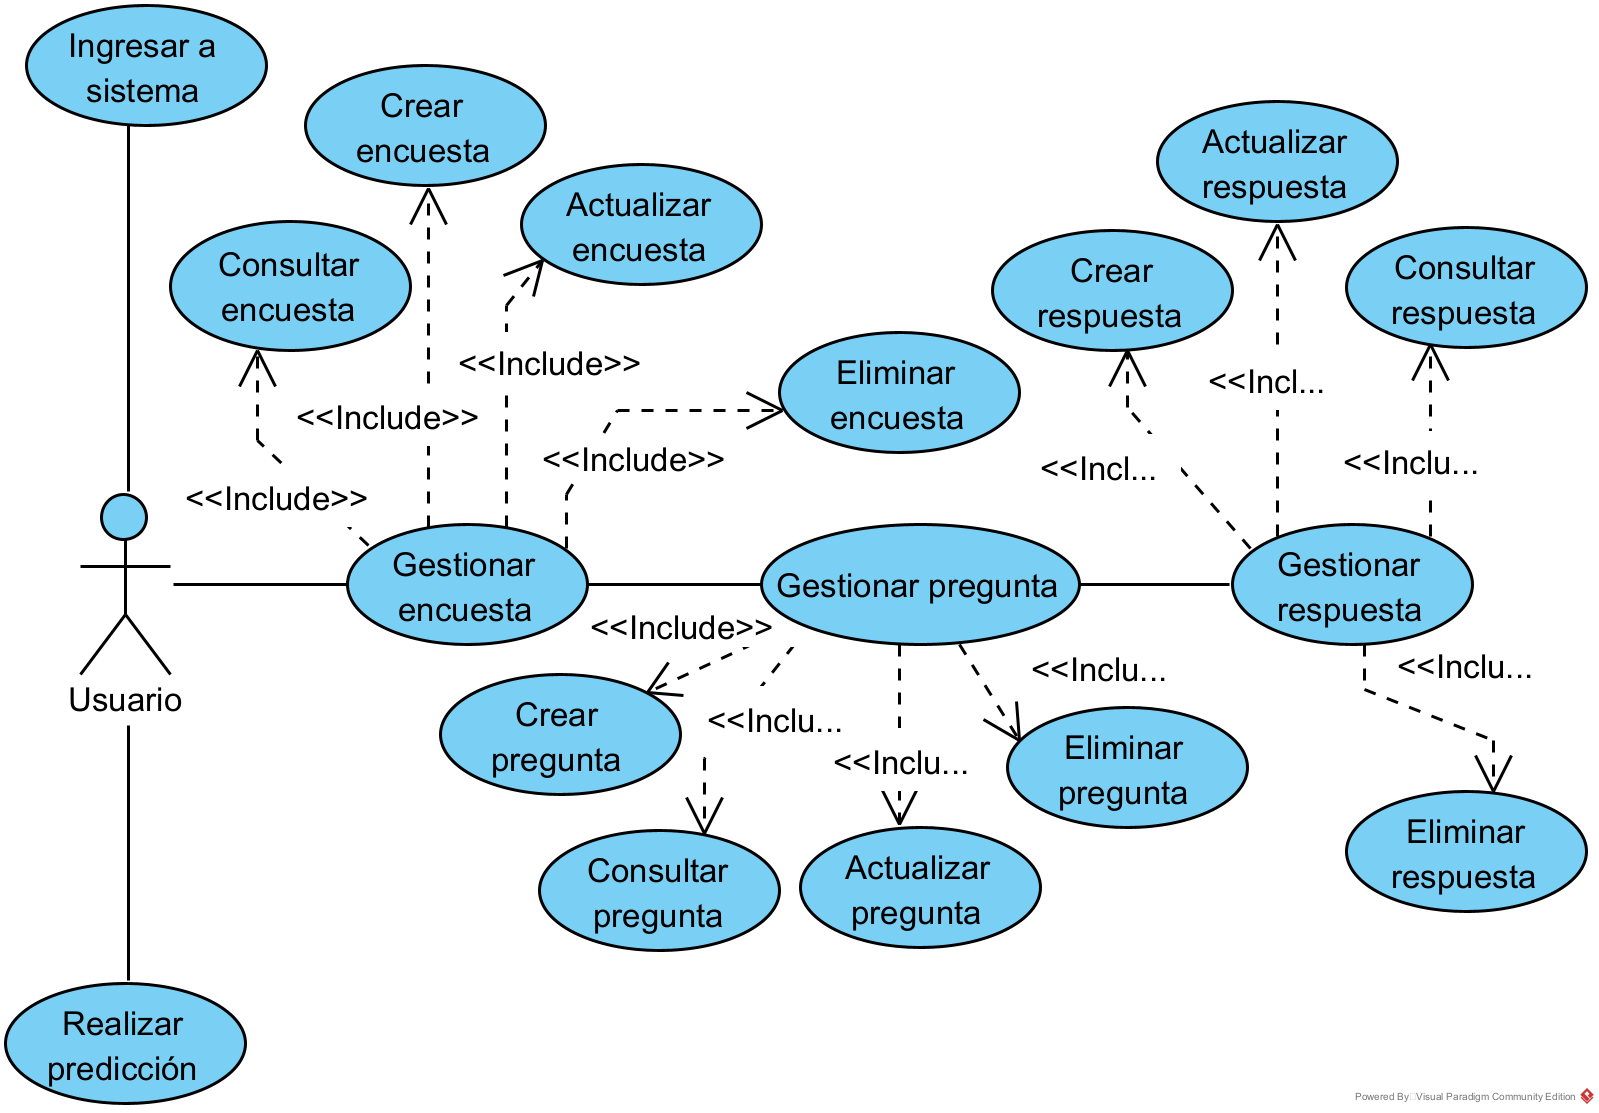
\includegraphics[scale=1.0]{TT/img/diseño/Crear encuesta.png}
    \caption{Diagrama de caso de uso sobre la gestión de encuestas }
    \label{graphic:CU-D-gestionar-encuesta}
\end{figure}


\subsection{Contestar encuesta}

\begin{figure}[!ht]
    \centering
    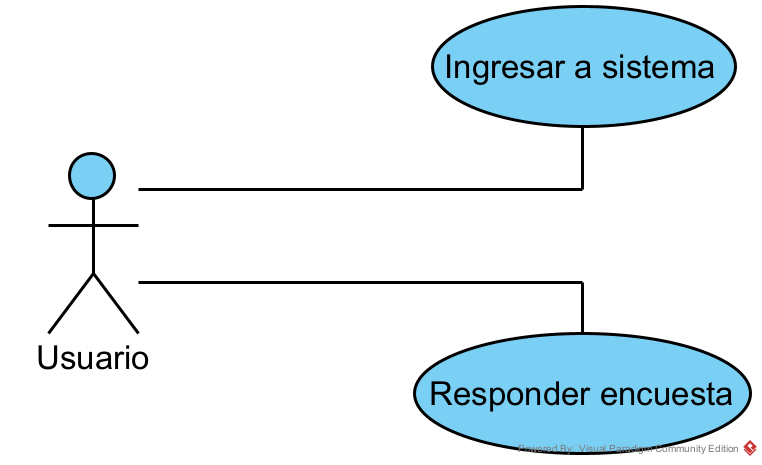
\includegraphics[scale=1.0]{TT/img/diseño/Responder encuesta.png}
    \caption{Diagrama de caso de uso sobre contestar encuesta}
    \label{graphic:CU-D-contestar-encuesta}
\end{figure}

\subsection{Opcional, manejar administrador de sistema}

\section{Especificación de casos de uso}

En esta sección se describen detalladamente todos los casos de uso del sistema.

\subsection{Ingresar al sistema}

\begin{longtable}{|>{\columncolor[HTML]{3531FF}}m{3cm}|m{11cm}|}
    \hline
    {\color[HTML]{FFFFFF} Caso de uso} & Ingresar sistema \\ \hline
    \endfirsthead
    \hline
    {\color[HTML]{FFFFFF} Caso de uso} & Ingresar sistema \\
    \hline 
    \endhead
    % aquí añadimos el fondo de todas las hojas, excepto de la última.
    \multicolumn{2}{c}{Sigue en la página siguiente.}
    \endfoot
    % aquí añadimos el fondo de la última hoja.
    \endlastfoot
    \hline
    {\color[HTML]{FFFFFF} Actores}& Usuario\\ \hline
    {\color[HTML]{FFFFFF} Resumen}& El usuario ingresa al sistema y se identifica\\ \hline
    {\color[HTML]{FFFFFF} Precondiciones}& Ninguna \\ \hline
    {\color[HTML]{FFFFFF} Flujo principal}& \begin{enumerate}
            \item El usuario se identifica mediante correo y contraseña e ingresa al modulo principal del sistema.
            \item Búsqueda de usuario existente.
            \item El sistema verifica que el usuario exista, el caso de uso termina.
        \end{enumerate}\\ \hline
    {\color[HTML]{FFFFFF} Subflujos}& \begin{enumerate}
        \item El usuario se identifica mediante correo y contraseña e ingresa al modulo principal del sistema.
    \end{enumerate}\\ \hline
    {\color[HTML]{FFFFFF} Excepciones}& \textbf{Usuario invalido:} El sistema informa que su usuario o contraseña no es correcto, el caso de uso termina.\\ \hline
    {\color[HTML]{FFFFFF} Postcondiciones}& \textbf{Usuario en sección correcta:} El usuario se encontrará en la parte del sistema que le corresponde.\\ \hline
    {\color[HTML]{FFFFFF} Escenarios de éxito}& \textbf{Un usuario ingresa al sistema:} El usuario ingresa correctamente al sistema.\\ \hline
    {\color[HTML]{FFFFFF} Escenarios de fracaso}& \textbf{Usuario identificado incorrectamente:} Usuario o contraseña inválido.\\ \hline
    \caption{Especificación de caso de uso de ingresar al sistema}
    \label{table:CU01}
\end{longtable}

\subsection{Crear encuesta}

\begin{longtable}{|>{\columncolor[HTML]{3531FF}}m{3cm}|m{11cm}|}
    \hline
    {\color[HTML]{FFFFFF} Caso de uso} & Crear encuesta\\ \hline
    \endfirsthead
    \hline
    {\color[HTML]{FFFFFF} Caso de uso} & Crear encuesta \\
    \hline 
    \endhead
    % aquí añadimos el fondo de todas las hojas, excepto de la última.
    \multicolumn{2}{c}{Sigue en la página siguiente.}
    \endfoot
    % aquí añadimos el fondo de la última hoja.
    \endlastfoot
    \hline
    {\color[HTML]{FFFFFF} Actores}& Usuario\\ \hline
    {\color[HTML]{FFFFFF} Resumen}& El usuario crea una encuesta que será almacenada en la base de datos.\\ \hline
    {\color[HTML]{FFFFFF} Precondiciones}& \textbf{Usuario identificado: }Usuario correctamente identificado \\ \hline
    {\color[HTML]{FFFFFF} Flujo principal}& \begin{enumerate}
            \item El usuario se dirige a la sección de encuestas.
            \item El usuario elige la opción de crear encuesta.
            \item El sistema muestra la pantalla para crear encuesta.
            \item El usuario ingresa los datos para crear encuesta.
            \item El usuario guarda la encuesta.
            \item El sistema guarda la encuesta en la base de datos, el caso de uso termina.
        \end{enumerate}\\ \hline
    {\color[HTML]{FFFFFF} Subflujos}& \textbf{Guardar encuesta}
    \begin{enumerate}
        \item El sistema verificará que todos los campos obligatorios se hayan llenado.
        \item El sistema guardará la encuesta en la base de datos.
    \end{enumerate}\\ \hline
    {\color[HTML]{FFFFFF} Excepciones}& \textbf{Guardar encuesta: }El sistema informará cuando la encuesta no se haya guardado correctamente.\\ \hline
    {\color[HTML]{FFFFFF} Postcondiciones}& \textbf{Encuesta almacenada: } La encuesta se almacena correctamente en la base de datos.\\ \hline
    {\color[HTML]{FFFFFF} Escenarios de éxito}& \textbf{La encuesta se almacena: }La encuesta se almacena exitosamente en la base de datos.\\ \hline
    {\color[HTML]{FFFFFF} Escenarios de fracaso}& \textbf{La encuesta no se almacena: }La encuesta no se almacena en la base de datos.\\ \hline
    \caption{Especificación de caso de uso de crear encuesta}
    \label{table:CU02}
\end{longtable}

\subsection{Consultar encuesta}

\begin{longtable}{|>{\columncolor[HTML]{3531FF}}m{3cm}|m{11cm}|}
    \hline
    {\color[HTML]{FFFFFF} Caso de uso} & Consultar encuesta \\ \hline
    \endfirsthead
    \hline
    {\color[HTML]{FFFFFF} Caso de uso} & Consultar encuesta \\
    \hline 
    \endhead
    % aquí añadimos el fondo de todas las hojas, excepto de la última.
    \multicolumn{2}{c}{Sigue en la página siguiente.}
    \endfoot
    % aquí añadimos el fondo de la última hoja.
    \endlastfoot
    \hline
    {\color[HTML]{FFFFFF} Actores}& Usuario\\ \hline
    {\color[HTML]{FFFFFF} Resumen}& El usuario consulta las encuestas creadas por el mismo.\\ \hline
    {\color[HTML]{FFFFFF} Precondiciones}& Usuario esta correctamente identificado \\ \hline
    {\color[HTML]{FFFFFF} Flujo principal}& \begin{enumerate}
            \item El usuario se dirige a la sección de encuestas.
            \item En la sección de encuestas, selecciona la opción de ver sus encuestas.
            \item El sistema muestra las encuestas creadas por el usuario.
        \end{enumerate}\\ \hline
    {\color[HTML]{FFFFFF} Subflujos}& Ninguno. \\ \hline
    {\color[HTML]{FFFFFF} Excepciones}& \textbf{Lista vacía: }No existen encuestas guardadas anteriormente.\\ \hline
    {\color[HTML]{FFFFFF} Postcondiciones}& \textbf{Encuestas mostradas:} Las encuestas correspondientes son mostradas correctamente.\\ \hline
    {\color[HTML]{FFFFFF} Escenarios de éxito}& \textbf{Las encuestas se muestran: } Las encuestas son mostradas al usuario.\\ \hline
    {\color[HTML]{FFFFFF} Escenarios de fracaso}& \textbf{Lista vacía:} Lista de encuestas vacías.\\ \hline
    \caption{Especificación de caso de uso de consultar encuesta}
    \label{table:CU04}
\end{longtable}

\subsection{Editar encuesta}

\begin{longtable}{|>{\columncolor[HTML]{3531FF}}m{3cm}|m{11cm}|}
    \hline
    {\color[HTML]{FFFFFF} Caso de uso} & Editar encuesta \\ \hline
    \endfirsthead
    \hline
    {\color[HTML]{FFFFFF} Caso de uso} & Editar encuesta \\
    \hline 
    \endhead
    % aquí añadimos el fondo de todas las hojas, excepto de la última.
    \multicolumn{2}{c}{Sigue en la página siguiente.}
    \endfoot
    % aquí añadimos el fondo de la última hoja.
    \endlastfoot
    \hline
    {\color[HTML]{FFFFFF} Actores}& Usuario\\ \hline
    {\color[HTML]{FFFFFF} Resumen}& El usuario modifica una encuesta existente creada por el mismo.\\ \hline
    {\color[HTML]{FFFFFF} Precondiciones}& El usuario esta correctamente identificado. \\ \hline
    {\color[HTML]{FFFFFF} Flujo principal}& \begin{enumerate}
            \item El usuario se dirige a la sección de encuestas.
            \item En la sección de encuestas, selecciona la opción de ver sus encuestas.
            \item El usuario selecciona una encuesta suya que va a modificar.
            \item Elige la opción de editar encuesta.
            \item El usuario modifica la encuesta seleccionada.
            \item El usuario guarda los cambios realizados en su encuesta, el caso de uso termina.
        \end{enumerate}\\ \hline
    {\color[HTML]{FFFFFF} Subflujos}& Ninguno. \\ \hline
    {\color[HTML]{FFFFFF} Excepciones}& \textbf{Lista vacía: }No existen encuestas guardadas anteriormente.\\ \hline
    {\color[HTML]{FFFFFF} Postcondiciones}& \textbf{Encuesta modificada: }La encuesta se ha modificado correctamente..\\ \hline
    {\color[HTML]{FFFFFF} Escenarios de éxito}& \textbf{La encuesta se modifica:} La encuesta se modifica correctamente.\\ \hline
    {\color[HTML]{FFFFFF} Escenarios de fracaso}& \textbf{La encuesta no se modifica:} La encuesta no se modifica correctamente.\\ \hline
    \caption{Especificación de caso de uso de editar encuesta}
    \label{table:CU03}
\end{longtable}

\subsection{Eliminar encuesta}

\begin{longtable}{|>{\columncolor[HTML]{3531FF}}m{3cm}|m{11cm}|}
    \hline
    {\color[HTML]{FFFFFF} Caso de uso} & Eliminar encuesta \\ \hline
    \endfirsthead
    \hline
    {\color[HTML]{FFFFFF} Caso de uso} & Eliminar encuesta \\
    \hline 
    \endhead
    % aquí añadimos el fondo de todas las hojas, excepto de la última.
    \multicolumn{2}{c}{Sigue en la página siguiente.}
    \endfoot
    % aquí añadimos el fondo de la última hoja.
    \endlastfoot
    \hline
    {\color[HTML]{FFFFFF} Actores}& Usuario\\ \hline
    {\color[HTML]{FFFFFF} Resumen}& El usuario elimina una encuesta\\ \hline
    {\color[HTML]{FFFFFF} Precondiciones}& Usuario esta correctamente identificado \\ \hline
    {\color[HTML]{FFFFFF} Flujo principal}& \begin{enumerate}
            \item El usuario se dirige a la sección de encuestas.
            \item En la sección de encuestas, selecciona la opción de ver sus encuestas.
            \item El sistema muestra las encuestas creadas por el usuario.
            \item El usuario selecciona la encuesta a eliminar.
            \item El usuario selecciona la opción de eliminar encuesta.
            \item El sistema le solicita la verificación de eliminación al usuario.
            \item El usuario acepta eliminar la encuesta.
            \item El sistema elimina la encuesta, el caso de uso termina.
        \end{enumerate}\\ \hline
    {\color[HTML]{FFFFFF} Subflujos}& Ninguno.\\ \hline
    {\color[HTML]{FFFFFF} Excepciones}& \textbf{Cancelación de la eliminación: }El usuario cancela la eliminación de la encuesta.\\ \hline
    {\color[HTML]{FFFFFF} Postcondiciones}& \textbf{Encuesta eliminada: }La encuesta es eliminada de la base de datos.\\ \hline
    {\color[HTML]{FFFFFF} Escenarios de éxito}& \textbf{La encuesta se elimina: }La pregunta se elimina correctamente de la base de datos.\\ \hline
    {\color[HTML]{FFFFFF} Escenarios de fracaso}& \textbf{La encuesta no se elimina: }La encuesta no se elimina de la base de datos.\\ \hline
    \caption{Especificación de caso de uso de eliminar encuesta}
    \label{table:CU05}
\end{longtable}

\subsection{Crear pregunta}

\begin{longtable}{|>{\columncolor[HTML]{3531FF}}m{3cm}|m{11cm}|}
    \hline
    {\color[HTML]{FFFFFF} Caso de uso} & Crear pregunta \\ \hline
    \endfirsthead
    \hline
    {\color[HTML]{FFFFFF} Caso de uso} & Crear pregunta \\
    \hline 
    \endhead
    % aquí añadimos el fondo de todas las hojas, excepto de la última.
    \multicolumn{2}{c}{Sigue en la página siguiente.}
    \endfoot
    % aquí añadimos el fondo de la última hoja.
    \endlastfoot
    \hline
    {\color[HTML]{FFFFFF} Actores}& Usuario\\ \hline
    {\color[HTML]{FFFFFF} Resumen}& El usuario crea una pregunta que será almacenada en la base de datos.\\ \hline
    {\color[HTML]{FFFFFF} Precondiciones}& \textbf{Usuario identificado: }Usuario correctamente identificado  y tiene que tener al menos una encuesta creada.\\ \hline
    {\color[HTML]{FFFFFF} Flujo principal}& \begin{enumerate}
            \item El usuario se dirige a la sección de encuestas.
            \item El usuario elige la opción de ver sus encuestas.
            \item El usuario elige la encuesta deseada para agregar preguntas.
            \item El sistema muestra la información de la encuesta.
            \item El usuario selección agregar pregunta.
            \item El usuario ingresa los datos para crear pregunta.
            \item El usuario guarda la pregunta.
            \item El sistema guarda la pregunta en la base de datos, el caso de uso termina.
        \end{enumerate}\\ \hline
    {\color[HTML]{FFFFFF} Subflujos}& \textbf{Guardar pregunta}
    \begin{enumerate}
        \item El sistema verificará que todos los campos obligatorios se hayan llenado.
        \item El sistema guardará la pregunta en la base de datos.
    \end{enumerate}\\ \hline
    {\color[HTML]{FFFFFF} Excepciones}& \textbf{Guardar pregunta: }El sistema informará cuando la pregunta no se haya guardado correctamente.\\ \hline
    {\color[HTML]{FFFFFF} Postcondiciones}& \textbf{Pregunta almacenada: } La pregunta se almacena correctamente en la base de datos.\\ \hline
    {\color[HTML]{FFFFFF} Escenarios de éxito}& \textbf{La pregunta se almacena: }La pregunta se almacena exitosamente en la base de datos.\\ \hline
    {\color[HTML]{FFFFFF} Escenarios de fracaso}& \textbf{La pregunta no se almacena: }La pregunta no se almacena en la base de datos.\\ \hline
    \caption{Especificación de caso de uso de crear pregunta}
    \label{table:CU06}
\end{longtable}

\subsection{Consultar pregunta}

\begin{longtable}{|>{\columncolor[HTML]{3531FF}}m{3cm}|m{11cm}|}
    \hline
    {\color[HTML]{FFFFFF} Caso de uso} & Consultar pregunta \\ \hline
    \endfirsthead
    \hline
    {\color[HTML]{FFFFFF} Caso de uso} & Consultar pregunta \\
    \hline 
    \endhead
    % aquí añadimos el fondo de todas las hojas, excepto de la última.
    \multicolumn{2}{c}{Sigue en la página siguiente.}
    \endfoot
    % aquí añadimos el fondo de la última hoja.
    \endlastfoot
    \hline
    {\color[HTML]{FFFFFF} Actores}& Usuario\\ \hline
     {\color[HTML]{FFFFFF} Resumen}& El usuario consulta las preguntas creadas por el mismo.\\ \hline
    {\color[HTML]{FFFFFF} Precondiciones}& Usuario esta correctamente identificado y tiene que tener al menos una encuesta creada.\\ \hline
    {\color[HTML]{FFFFFF} Flujo principal}& \begin{enumerate}
            \item El usuario se dirige a la sección de encuestas.
            \item El usuario elige la opción de ver sus encuestas.
            \item El usuario elige la encuesta deseada.
            \item El sistema muestra la información de la encuesta junto con sus preguntas.
        \end{enumerate}\\ \hline
    {\color[HTML]{FFFFFF} Subflujos}& Ninguno. \\ \hline
    {\color[HTML]{FFFFFF} Excepciones}& \textbf{Lista vacía: }No existen preguntas guardadas anteriormente.\\ \hline
    {\color[HTML]{FFFFFF} Postcondiciones}& \textbf{Preguntas mostradas:} Las preguntas correspondientes son mostradas correctamente.\\ \hline
    {\color[HTML]{FFFFFF} Escenarios de éxito}& \textbf{Las preguntas se muestran: } Las preguntas son mostradas al usuario.\\ \hline
    {\color[HTML]{FFFFFF} Escenarios de fracaso}& \textbf{Lista vacía:} Lista de preguntas vacías.\\ \hline
    \caption{Especificación de caso de uso de consultar pregunta}
    \label{table:CU08}
\end{longtable}

\subsection{Editar pregunta}

\begin{longtable}{|>{\columncolor[HTML]{3531FF}}m{3cm}|m{11cm}|}
    \hline
    {\color[HTML]{FFFFFF} Caso de uso} & Editar pregunta \\ \hline
    \endfirsthead
    \hline
    {\color[HTML]{FFFFFF} Caso de uso} & Editar pregunta \\
    \hline 
    \endhead
    % aquí añadimos el fondo de todas las hojas, excepto de la última.
    \multicolumn{2}{c}{Sigue en la página siguiente.}
    \endfoot
    % aquí añadimos el fondo de la última hoja.
    \endlastfoot
    \hline
    {\color[HTML]{FFFFFF} Actores}& Usuario\\ \hline
    {\color[HTML]{FFFFFF} Resumen}& El usuario modifica una pregunta existente de una encuesta creada por el mismo.\\ \hline
    {\color[HTML]{FFFFFF} Precondiciones}& El usuario esta correctamente identificado  y tiene que tener al menos una encuesta creada. \\ \hline
    {\color[HTML]{FFFFFF} Flujo principal}& \begin{enumerate}
            \item El usuario se dirige a la sección de encuestas.
            \item El usuario elige la opción de ver sus encuestas.
            \item El usuario elige la encuesta deseada.
            \item El sistema muestra la información de la encuesta junto con sus preguntas.
            \item El sistema muestra la información de la encuesta.
            \item El usuario selecciona una pregunta suya que va a modificar.
            \item Elige la opción de editar pregunta.
            \item El usuario modifica la pregunta seleccionada.
            \item El usuario guarda los cambios realizados en su pregunta, el caso de uso termina.
        \end{enumerate}\\ \hline
    {\color[HTML]{FFFFFF} Subflujos}& Ninguno. \\ \hline
    {\color[HTML]{FFFFFF} Excepciones}& \textbf{Lista vacía: }No existen preguntas guardadas anteriormente.\\ \hline
    {\color[HTML]{FFFFFF} Postcondiciones}& \textbf{Pregunta modificada: }La pregunta se ha modificado correctamente.\\ \hline
    {\color[HTML]{FFFFFF} Escenarios de éxito}& \textbf{La pregunta se modifica:} La pregunta se modifica correctamente.\\ \hline
    {\color[HTML]{FFFFFF} Escenarios de fracaso}& \textbf{La pregunta no se modifica:} La pregunta no se modifica correctamente.\\ \hline
    \caption{Especificación de caso de uso de editar pregunta}
    \label{table:CU07}
\end{longtable}

\subsection{Eliminar pregunta}

\begin{longtable}{|>{\columncolor[HTML]{3531FF}}m{3cm}|m{11cm}|}
    \hline
    {\color[HTML]{FFFFFF} Caso de uso} & Eliminar pregunta \\ \hline
    \endfirsthead
    \hline
    {\color[HTML]{FFFFFF} Caso de uso} & Eliminar pregunta \\
    \hline 
    \endhead
    % aquí añadimos el fondo de todas las hojas, excepto de la última.
    \multicolumn{2}{c}{Sigue en la página siguiente.}
    \endfoot
    % aquí añadimos el fondo de la última hoja.
    \endlastfoot
    \hline
    {\color[HTML]{FFFFFF} Actores}& Usuario\\ \hline
    {\color[HTML]{FFFFFF} Resumen}& El usuario elimina una pregunta de una encuesta creada por el mismo\\ \hline
    {\color[HTML]{FFFFFF} Precondiciones}& Usuario esta correctamente identificado  y tiene que tener al menos una encuesta creada.\\ \hline
    {\color[HTML]{FFFFFF} Flujo principal}& \begin{enumerate}
            \item El usuario se dirige a la sección de encuestas.
            \item El usuario elige la opción de ver sus encuestas.
            \item El usuario elige la encuesta deseada.
            \item El sistema muestra la información de la encuesta junto con sus preguntas.
            \item El sistema muestra la información de la encuesta junto con sus preguntas.
            \item El usuario selecciona una pregunta suya que va a eliminar.
            \item Elige la opción de eliminar pregunta.
            \item El usuario elimina la pregunta seleccionada.
            \item El sistema le notifica al usuario sobre la eliminación de la pregunta.
            \item El usuario confirma la eliminación de su pregunta.
            \item El sistema elimina la pregunta de la base de datos.
        \end{enumerate}\\ \hline
    {\color[HTML]{FFFFFF} Subflujos}& Ninguno.\\ \hline
    {\color[HTML]{FFFFFF} Excepciones}& \textbf{Cancelación de la eliminación: }El usuario cancela la eliminación de la pregunta.\\ \hline
    {\color[HTML]{FFFFFF} Postcondiciones}& \textbf{Pregunta eliminada: }La pregunta es eliminada de la base de datos.\\ \hline
    {\color[HTML]{FFFFFF} Escenarios de éxito}& \textbf{La Pregunta se elimina: }La pregunta se elimina correctamente de la base de datos.\\ \hline
    {\color[HTML]{FFFFFF} Escenarios de fracaso}& \textbf{La pregunta no se elimina: }La pregunta no se elimina de la base de datos.\\ \hline
    \caption{Especificación de caso de uso de Eliminar pregunta}
    \label{table:CU09}
\end{longtable}

\subsection{Crear respuesta}

\begin{longtable}{|>{\columncolor[HTML]{3531FF}}m{3cm}|m{11cm}|}
    \hline
    {\color[HTML]{FFFFFF} Caso de uso} & Crear respuesta \\ \hline
    \endfirsthead
    \hline
    {\color[HTML]{FFFFFF} Caso de uso} & Crear respuesta \\
    \hline 
    \endhead
    % aquí añadimos el fondo de todas las hojas, excepto de la última.
    \multicolumn{2}{c}{Sigue en la página siguiente.}
    \endfoot
    % aquí añadimos el fondo de la última hoja.
    \endlastfoot
    \hline
    {\color[HTML]{FFFFFF} Actores}& Usuario\\ \hline
    {\color[HTML]{FFFFFF} Resumen}& El usuario crea una respuesta para una pregunta de una encuesta que será almacenada en la base de datos.\\ \hline
    {\color[HTML]{FFFFFF} Precondiciones}& \textbf{Usuario identificado: }Usuario correctamente identificado  y tiene que tener al menos una encuesta creada con al menos una pregunta creada.\\ \hline
    {\color[HTML]{FFFFFF} Flujo principal}& \begin{enumerate}
            \item El usuario se dirige a la sección de encuestas.
            \item El usuario elige la opción de ver sus encuestas.
            \item El usuario elige la encuesta deseada para agregar preguntas.
            \item El sistema muestra la información de la encuesta.
            \item El usuario selecciona una pregunta.
            \item El usuario selecciona agregar una opción.
            \item El usuario ingresa los datos para crear una opción de respuesta.
            \item El usuario guarda la opción de respuesta.
            \item El sistema guarda la opción de respuesta en la base de datos, el caso de uso termina.
        \end{enumerate}\\ \hline
    {\color[HTML]{FFFFFF} Subflujos}& \textbf{Guardar opción de respuesta}
    \begin{enumerate}
        \item El sistema verificará que todos los campos obligatorios se hayan llenado.
        \item El sistema guardará la pregunta en la base de datos.
    \end{enumerate}\\ \hline
    {\color[HTML]{FFFFFF} Excepciones}& \textbf{Guardar pregunta: }El sistema informará cuando la pregunta no se haya guardado correctamente.
    \\ \hline
    {\color[HTML]{FFFFFF} Postcondiciones}& \textbf{Opción de respuesta almacenada: } La opción se almacena correctamente en la base de datos.\\ \hline
    {\color[HTML]{FFFFFF} Escenarios de éxito}& \textbf{La opción se almacena: }La opción se almacena exitosamente en la base de datos.\\ \hline
    {\color[HTML]{FFFFFF} Escenarios de fracaso}& \textbf{La opción no se almacena: }La opción no se almacena en la base de datos.\\ \hline
    \caption{Especificación de caso de uso de crear respuesta}
    \label{table:CU10}
\end{longtable}

\subsection{Consultar respuesta}

\begin{longtable}{|>{\columncolor[HTML]{3531FF}}m{3cm}|m{11cm}|}
    \hline
    {\color[HTML]{FFFFFF} Caso de uso} & Consultar respuesta \\ \hline
    \endfirsthead
    \hline
    {\color[HTML]{FFFFFF} Caso de uso} & Consultar respuesta \\
    \hline 
    \endhead
    % aquí añadimos el fondo de todas las hojas, excepto de la última.
    \multicolumn{2}{c}{Sigue en la página siguiente.}
    \endfoot
    % aquí añadimos el fondo de la última hoja.
    \endlastfoot
    \hline
    {\color[HTML]{FFFFFF} Actores}& Usuario\\ \hline
     {\color[HTML]{FFFFFF} Resumen}& El usuario consulta las preguntas creadas por el mismo.\\ \hline
    {\color[HTML]{FFFFFF} Precondiciones}& Usuario esta correctamente identificado y tiene que tener al menos una encuesta creada.\\ \hline
    {\color[HTML]{FFFFFF} Flujo principal}& \begin{enumerate}
            \item El usuario se dirige a la sección de encuestas.
            \item El usuario elige la opción de ver sus encuestas.
            \item El usuario elige la encuesta deseada.
            \item El sistema muestra la información de la encuesta junto con sus preguntas.
            \item El usuario visualiza todas las preguntas con sus opciones de respuesta de la encuesta seleccionada.
        \end{enumerate}\\ \hline
    {\color[HTML]{FFFFFF} Subflujos}& Ninguno. \\ \hline
    {\color[HTML]{FFFFFF} Excepciones}& \textbf{Lista vacía: }No existen preguntas guardadas anteriormente.\\ \hline
    {\color[HTML]{FFFFFF} Postcondiciones}& \textbf{Preguntas mostradas:} Las preguntas correspondientes son mostradas correctamente.\\ \hline
    {\color[HTML]{FFFFFF} Escenarios de éxito}& \textbf{Las preguntas se muestran: } Las preguntas son mostradas al usuario.\\ \hline
    {\color[HTML]{FFFFFF} Escenarios de fracaso}& \textbf{Lista vacía:} Lista de preguntas vacías.\\ \hline
    \caption{Especificación de caso de uso de consultar respuesta}
    \label{table:CU12}
\end{longtable}

\subsection{Editar respuesta}

\begin{longtable}{|>{\columncolor[HTML]{3531FF}}m{3cm}|m{11cm}|}
    \hline
    {\color[HTML]{FFFFFF} Caso de uso} & Editar respuesta \\ \hline
    \endfirsthead
    \hline
    {\color[HTML]{FFFFFF} Caso de uso} & Editar respuesta \\
    \hline 
    \endhead
    % aquí añadimos el fondo de todas las hojas, excepto de la última.
    \multicolumn{2}{c}{Sigue en la página siguiente.}
    \endfoot
    % aquí añadimos el fondo de la última hoja.
    \endlastfoot
    \hline
    {\color[HTML]{FFFFFF} Actores}& Usuario\\ \hline
    {\color[HTML]{FFFFFF} Resumen}& El usuario modifica una opción de respuesta existente de una encuesta creada por el mismo.\\ \hline
    {\color[HTML]{FFFFFF} Precondiciones}& El usuario esta correctamente identificado  y tiene que tener al menos una encuesta creada con una pregunta creada. \\ \hline
    {\color[HTML]{FFFFFF} Flujo principal}& \begin{enumerate}
            \item El usuario se dirige a la sección de encuestas.
            \item El usuario elige la opción de ver sus encuestas.
            \item El usuario elige la encuesta deseada.
            \item El sistema muestra la información de la encuesta junto con sus preguntas.
            \item El sistema muestra la información de la encuesta.
            \item El usuario selecciona una pregunta para editar sus respuestas.
            \item Elige la opción de editar la respuesta.
            \item El usuario modifica la respuesta seleccionada.
            \item El usuario guarda los cambios realizados en su opción de respuesta, el caso de uso termina.
        \end{enumerate}\\ \hline
    {\color[HTML]{FFFFFF} Subflujos}& Ninguno. \\ \hline
    {\color[HTML]{FFFFFF} Excepciones}& \textbf{Lista vacía: }No existen opciones de respuestas guardadas anteriormente.\\ \hline
    {\color[HTML]{FFFFFF} Postcondiciones}& \textbf{Opción de respuesta modificada: }La pregunta se ha modificado correctamente.\\ \hline
    {\color[HTML]{FFFFFF} Escenarios de éxito}& \textbf{La opción de respuesta se modifica:} La opción de respuesta se modifica correctamente.\\ \hline
    {\color[HTML]{FFFFFF} Escenarios de fracaso}& \textbf{La opción de respuesta no se modifica:} La opción de respuesta no se modifica correctamente.\\ \hline
    \caption{Especificación de caso de uso de editar opción de respuesta}
    \label{table:CU11}
\end{longtable}

\subsection{Eliminar respuesta}

\begin{longtable}{|>{\columncolor[HTML]{3531FF}}m{3cm}|m{11cm}|}
    \hline
    {\color[HTML]{FFFFFF} Caso de uso} & Eliminar respuesta \\ \hline
    \endfirsthead
    \hline
    {\color[HTML]{FFFFFF} Caso de uso} & Eliminar respuesta \\
    \hline 
    \endhead
    % aquí añadimos el fondo de todas las hojas, excepto de la última.
    \multicolumn{2}{c}{Sigue en la página siguiente.}
    \endfoot
    % aquí añadimos el fondo de la última hoja.
    \endlastfoot
    \hline
    {\color[HTML]{FFFFFF} Actores}& Usuario\\ \hline
    {\color[HTML]{FFFFFF} Resumen}& El usuario elimina una opción de respuesta de una pregunta de la encuesta creada por el mismo\\ \hline
    {\color[HTML]{FFFFFF} Precondiciones}& Usuario esta correctamente identificado  y tiene que tener al menos una encuesta con una pregunta creada .\\ \hline
    {\color[HTML]{FFFFFF} Flujo principal}& \begin{enumerate}
            \item El usuario se dirige a la sección de encuestas.
            \item El usuario elige la opción de ver sus encuestas.
            \item El usuario elige la encuesta deseada.
            \item El sistema muestra la información de la encuesta junto con sus preguntas.
            \item El sistema muestra la información de la encuesta junto con sus preguntas.
            \item EL usuario selecciona una pregunta.
            \item El usuario selecciona una opción de respuesta que va a eliminar.
            \item Elige la opción de eliminar respuesta.
            \item El usuario elimina la respuesta seleccionada.
            \item El sistema le notifica al usuario sobre la eliminación de la respuesta.
            \item El usuario confirma la eliminación de su respuesta.
            \item El sistema elimina la opción de respuesta de la base de datos.
        \end{enumerate}\\ \hline
    {\color[HTML]{FFFFFF} Subflujos}& Ninguno.\\ \hline
    {\color[HTML]{FFFFFF} Excepciones}& \textbf{Cancelación de la eliminación: }El usuario cancela la eliminación de la opción de respuesta.\\ \hline
    {\color[HTML]{FFFFFF} Postcondiciones}& \textbf{Opción de respuesta eliminada: }La opción de respuesta es eliminada de la base de datos.\\ \hline
    {\color[HTML]{FFFFFF} Escenarios de éxito}& \textbf{La opción de respuesta se elimina: }La opción de respuesta se elimina correctamente de la base de datos.\\ \hline
    {\color[HTML]{FFFFFF} Escenarios de fracaso}& \textbf{La opción de respuesta no se elimina: }La opción de respuesta no se elimina de la base de datos.\\ \hline
    \caption{Especificación de caso de uso de eliminar respuesta}
    \label{table:CU13}
\end{longtable}

\subsection{Responder encuesta}

\begin{longtable}{|>{\columncolor[HTML]{3531FF}}m{3cm}|m{11cm}|}
    \hline
    {\color[HTML]{FFFFFF} Caso de uso} & Responder encuesta\\ \hline
    \endfirsthead
    \hline
    {\color[HTML]{FFFFFF} Caso de uso} & Responder encuesta \\
    \hline 
    \endhead
    % aquí añadimos el fondo de todas las hojas, excepto de la última.
    \multicolumn{2}{c}{Sigue en la página siguiente.}
    \endfoot
    % aquí añadimos el fondo de la última hoja.
    \endlastfoot
    \hline
    {\color[HTML]{FFFFFF} Actores}& Usuario\\ \hline
    {\color[HTML]{FFFFFF} Resumen}& El usuario responde a una encuesta en la base de datos.\\ \hline
    {\color[HTML]{FFFFFF} Precondiciones}& Usuario correctamente identificado. \\ \hline
    {\color[HTML]{FFFFFF} Flujo principal}& \begin{enumerate}
            \item El usuario ingresa al módulo de encuestas.
            \item El usuario selecciona la encuesta que desea contestar.
            \item El sistema le muestra la encuesta.
            \item El usuario responde la encuesta con base a su opinión.
            \item El usuario al terminar, selecciona la opción de guardar encuesta.
            \item El sistema guarda su respuesta en la base de datos, el caso de uso termina.
        \end{enumerate}\\ \hline
    {\color[HTML]{FFFFFF} Subflujos}& Ninguno\\ \hline
    {\color[HTML]{FFFFFF} Excepciones}& \textbf{Respuesta no guardada: }El usuario no guarda su respuesta en el sistema.\\ \hline
    {\color[HTML]{FFFFFF} Postcondiciones}& \textbf{Resultados almacenados: }Los resultados se almacenan en la base de datos.\\ \hline
    {\color[HTML]{FFFFFF} Escenarios de éxito}& \textbf{Los resultados se almacenan: }Los resultados de la encuesta se almacenan correctamente en la base de datos.\\ \hline
    {\color[HTML]{FFFFFF} Escenarios de fracaso}& \textbf{Los resultados no se almacenan: }Los resultados de la encuesta no almacenan en la base de datos.\\ \hline
    \caption{Especificación de caso de uso de responder encuesta}
    \label{table:CU14}
\end{longtable}

\subsection{Realizar predicción}

\begin{longtable}{|>{\columncolor[HTML]{3531FF}}m{3cm}|m{11cm}|}
    \hline
    {\color[HTML]{FFFFFF} Caso de uso} & Realizar predicción\\ \hline
    \endfirsthead
    \hline
    {\color[HTML]{FFFFFF} Caso de uso} & Realizar predicción \\
    \hline 
    \endhead
    % aquí añadimos el fondo de todas las hojas, excepto de la última.
    \multicolumn{2}{c}{Sigue en la página siguiente.}
    \endfoot
    % aquí añadimos el fondo de la última hoja.
    \endlastfoot
    \hline
    {\color[HTML]{FFFFFF} Actores}& Usuario\\ \hline
    {\color[HTML]{FFFFFF} Resumen}& El usuario elige la opción de realizar predicción, se le preguntará si desea tomar en cuenta los valores existentes en la base de datos o bien cargar los datos directamente, es decir, el porcentaje de aceptación inicial.\\ \hline
    {\color[HTML]{FFFFFF} Precondiciones}& Usuario correctamente identificado\\ \hline
    {\color[HTML]{FFFFFF} Flujo principal}& \begin{enumerate}
            \item El usuario se dirige a la sección de encuestas.
            \item El usuario selecciona el menú de sus encuestas.
            \item El usuario selecciona una encuesta creada por el mismo.
            \item El usuario elige la opción de realizar predicción.
            \item El político decide usar los valores existentes en la base de datos para realizar la predicción.
            \item El sistema realizará el cálculo de predicción.
            \item El sistema mostrará los resultados.
        \end{enumerate}\\ \hline
    {\color[HTML]{FFFFFF} Subflujos}& El político puede optar por utilizar sus propios porcentajes iniciales y población, estos valores serán solicitados por el sistema.\\ \hline
    {\color[HTML]{FFFFFF} Excepciones}& \textbf{No hay respuestas en la base de datos: }Al no existir respuestas en la base de datos no se puede realizar una predicción.\\ \hline
    {\color[HTML]{FFFFFF} Postcondiciones}& \textbf{Usuario en sección correcta: }La predicción se realiza con éxito.\\ \hline
    {\color[HTML]{FFFFFF} Escenarios de éxito}& \textbf{La predicción se realiza: }La predicción se realiza con éxito.\\ \hline
    {\color[HTML]{FFFFFF} Escenarios de fracaso}& \textbf{La predicción no se realiza: }No se realiza una predicción.\\ \hline
    \caption{Especificación de caso de uso de realizar predicción}
    \label{table:CU15}
\end{longtable}

\section{Diagramas de secuencia}
Un diagrama de secuencia muestra la interacción de un conjunto de objetos en una aplicación a través del tiempo y se modela para cada caso de uso.

A continuación se muestran los diagramas de secuencia necesarios por cada caso de uso referentes al módulo de predicción.

\subsection{Realizar predicción}

\begin{figure}[!ht]
    \centering
    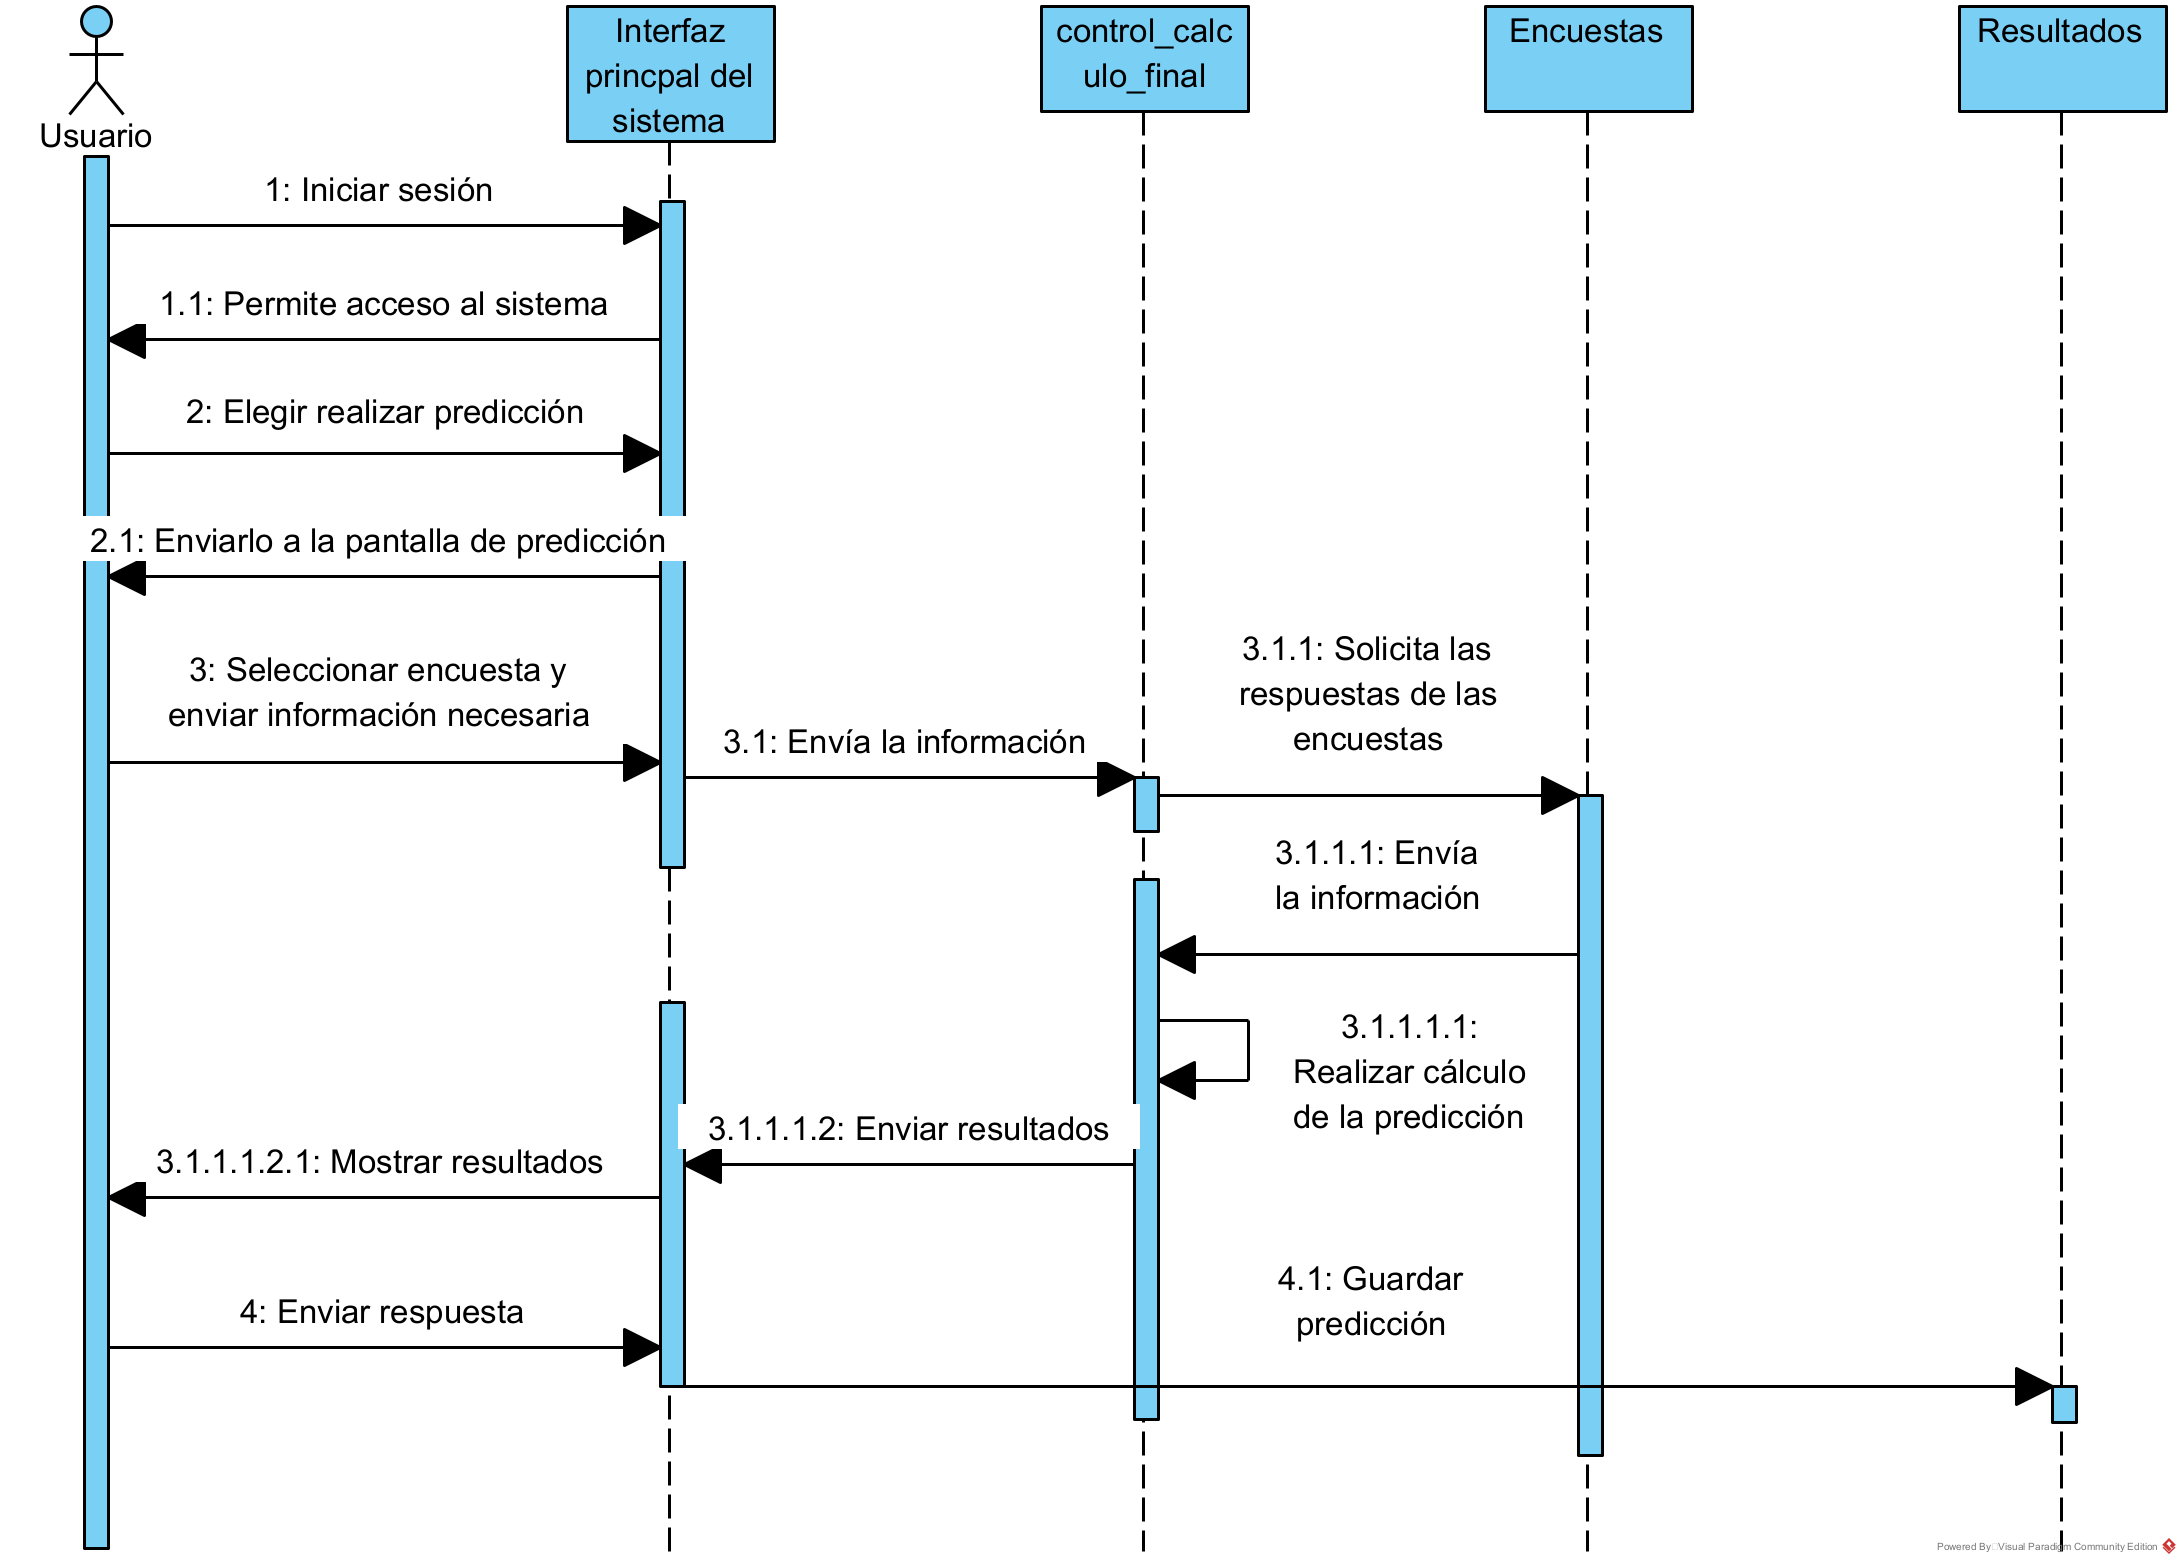
\includegraphics[scale=0.850]{TT/img/diseño/Realizar predicción.png}
    \caption{Diagrama de secuencia: Realizar predicción}
    \label{graphic:DS-Realizar predicción}
\end{figure}

\subsubsection{Descripción del flujo de información}

\begin{enumerate}
    \item Para realizar la predicción el usuario ingresa al sistema con su usuario y contraseña.
    \item El sistema verificará que los datos ingresados sean correctos, de ser así, permite el acceso al sistema.
    \item El usuario navegará a la sección de realizar predicción.
    \item El sistema le mostrará la página para realizar la predicción.
    \item El usuario seleccionará alguna encuesta creada por él y llenará los campos necesarios para realizar la predicción.
    \item La información enviada a través de la interfaz, será transferida al modulo de cálculo de predicción del servidor.
    \item El módulo de predicción solicita las respuestas de la encuesta a la base de datos.
    \item La base de datos envía las respuestas de la encuesta solicitadas.
    \item El módulo hará la predicción con los datos proporcionados.
    \item Los resultados son enviados a la interfaz gráfica.
    \item La interfaz desplegará la información recibida al usuario.
    \item El usuario decidirá si desea guardar los resultados en la base de datos o de lo contrario puede volver al paso 5.
    \item Si el usuario decidió guardar los resultados, estos se guardarán en la base de datos.
\end{enumerate}

\section{Diagramas de estado}

\subsection{Realizar predicción}
El diagrama siguiente muestra la transición de estados que se da al momento de realizar el cálculo de la predicción, el nodo negro representa el punto inicial.

\begin{figure}[!ht]
    \centering
    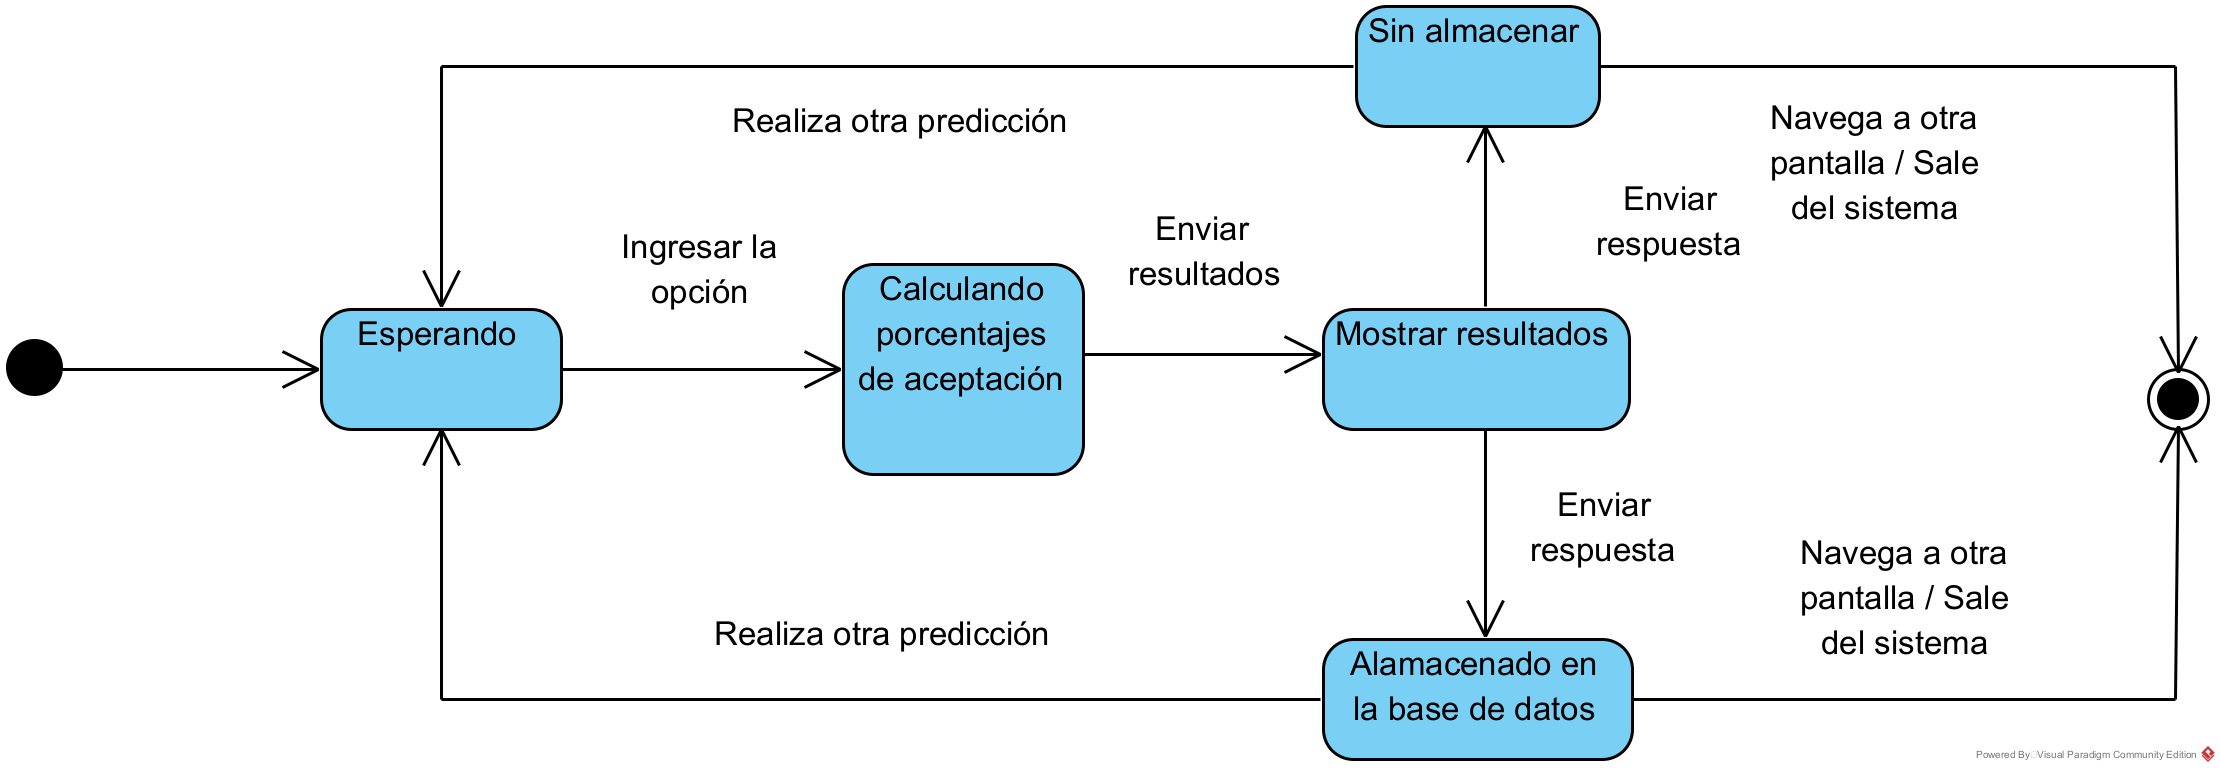
\includegraphics[scale=0.850]{TT/img/diseño/Realizar predicción DS.png}
    \caption{Diagrama de estado: Realizar predicción}
    \label{graphic:DE-Realizar predicción}
\end{figure}

\subsubsection{Descripción de estados: Realizar predicción}
\begin{enumerate}
    \item \textbf{Esperando: }En este estado, la interfaz gráfica de usuario espera a que el usuario elija una opción para la predicción.
    \item \textbf{Calculando porcentajes de aceptación: }Se calculan los porcentajes de éxito y fracaso.
    \item \textbf{Mostrar resultados: }El módulo de control envía los resultados a la interfaz gráfica y esta los muestra.
    \item \textbf{Sin almacenar: }No se almacenan los datos en la base de datos.
    \item \textbf{Almacenado en la base de datos: }Los datos son guardados.
    \item El ciclo de estados termina volviendo a realizar una predicción o saliendo de la pantalla de predicción o del sistema.
\end{enumerate}

\section{Diagrama de actividades}

\subsection{Realizar predicción}
El siguiente diagrama muestran las actividades que se realizan en el cálculo de la predicción así como el control de su flujo. El nodo negro indica un inicio y el nodo negro encerrado dentro de otra circunferencia indica el punto final.

\begin{figure}[!ht]
    \centering
    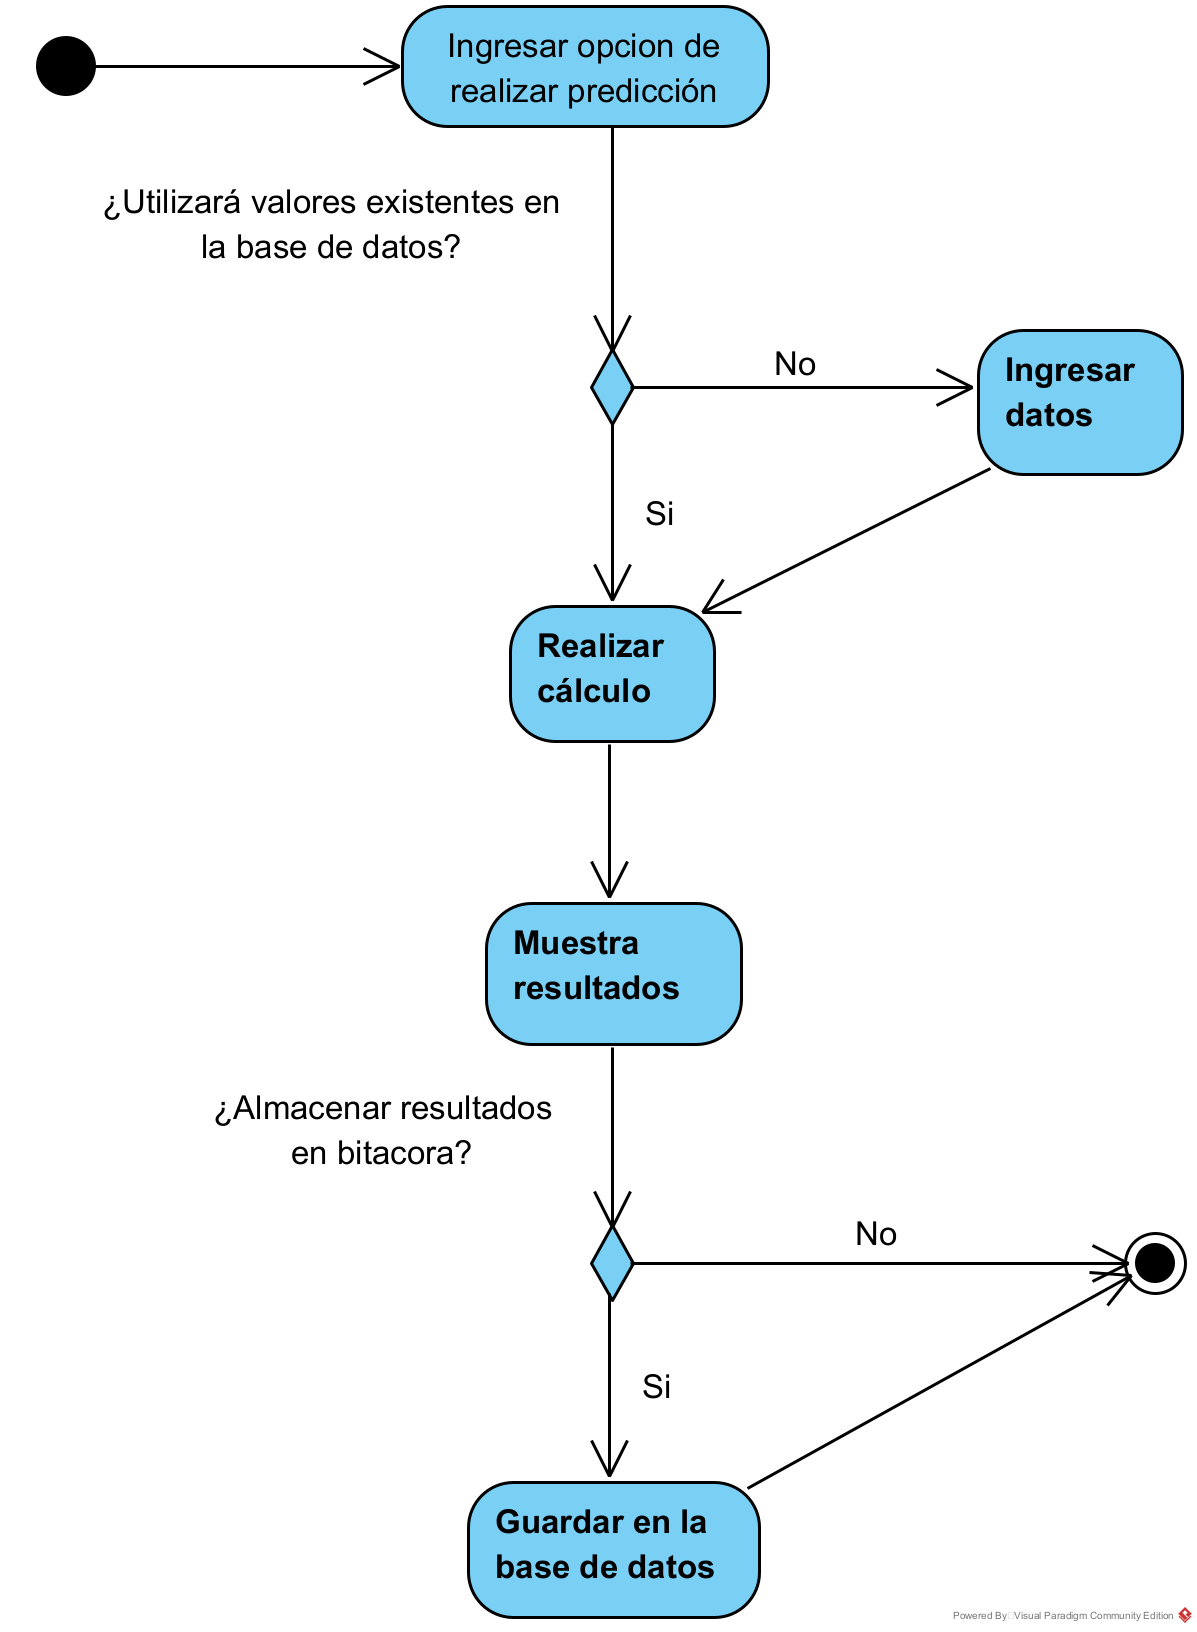
\includegraphics[scale=0.850]{TT/img/diseño/Realizar predicción DA.png}
    \caption{Diagrama de actividad: Realizar predicción}
    \label{graphic:DA-Realizar predicción}
\end{figure}

%\section{Diagrama de clases}

%\subsection{Tipos de clases}

%\subsection{Clases de entidad}

%\subsection{Clases de frontera}

%\subsection{Clases de control}

\section{Diseño de bases de datos}
Para el funcionamiento de este sistema será necesaria la implementación de una base de datos, para guardar los datos de los usuarios, las encuestas y sus respuestas.

\subsection{Diagrama de entidad relación}
SISPREL guardará los datos que están en el siguiente diagrama de entidad-relación.

\begin{figure}[!ht]
    \centering
    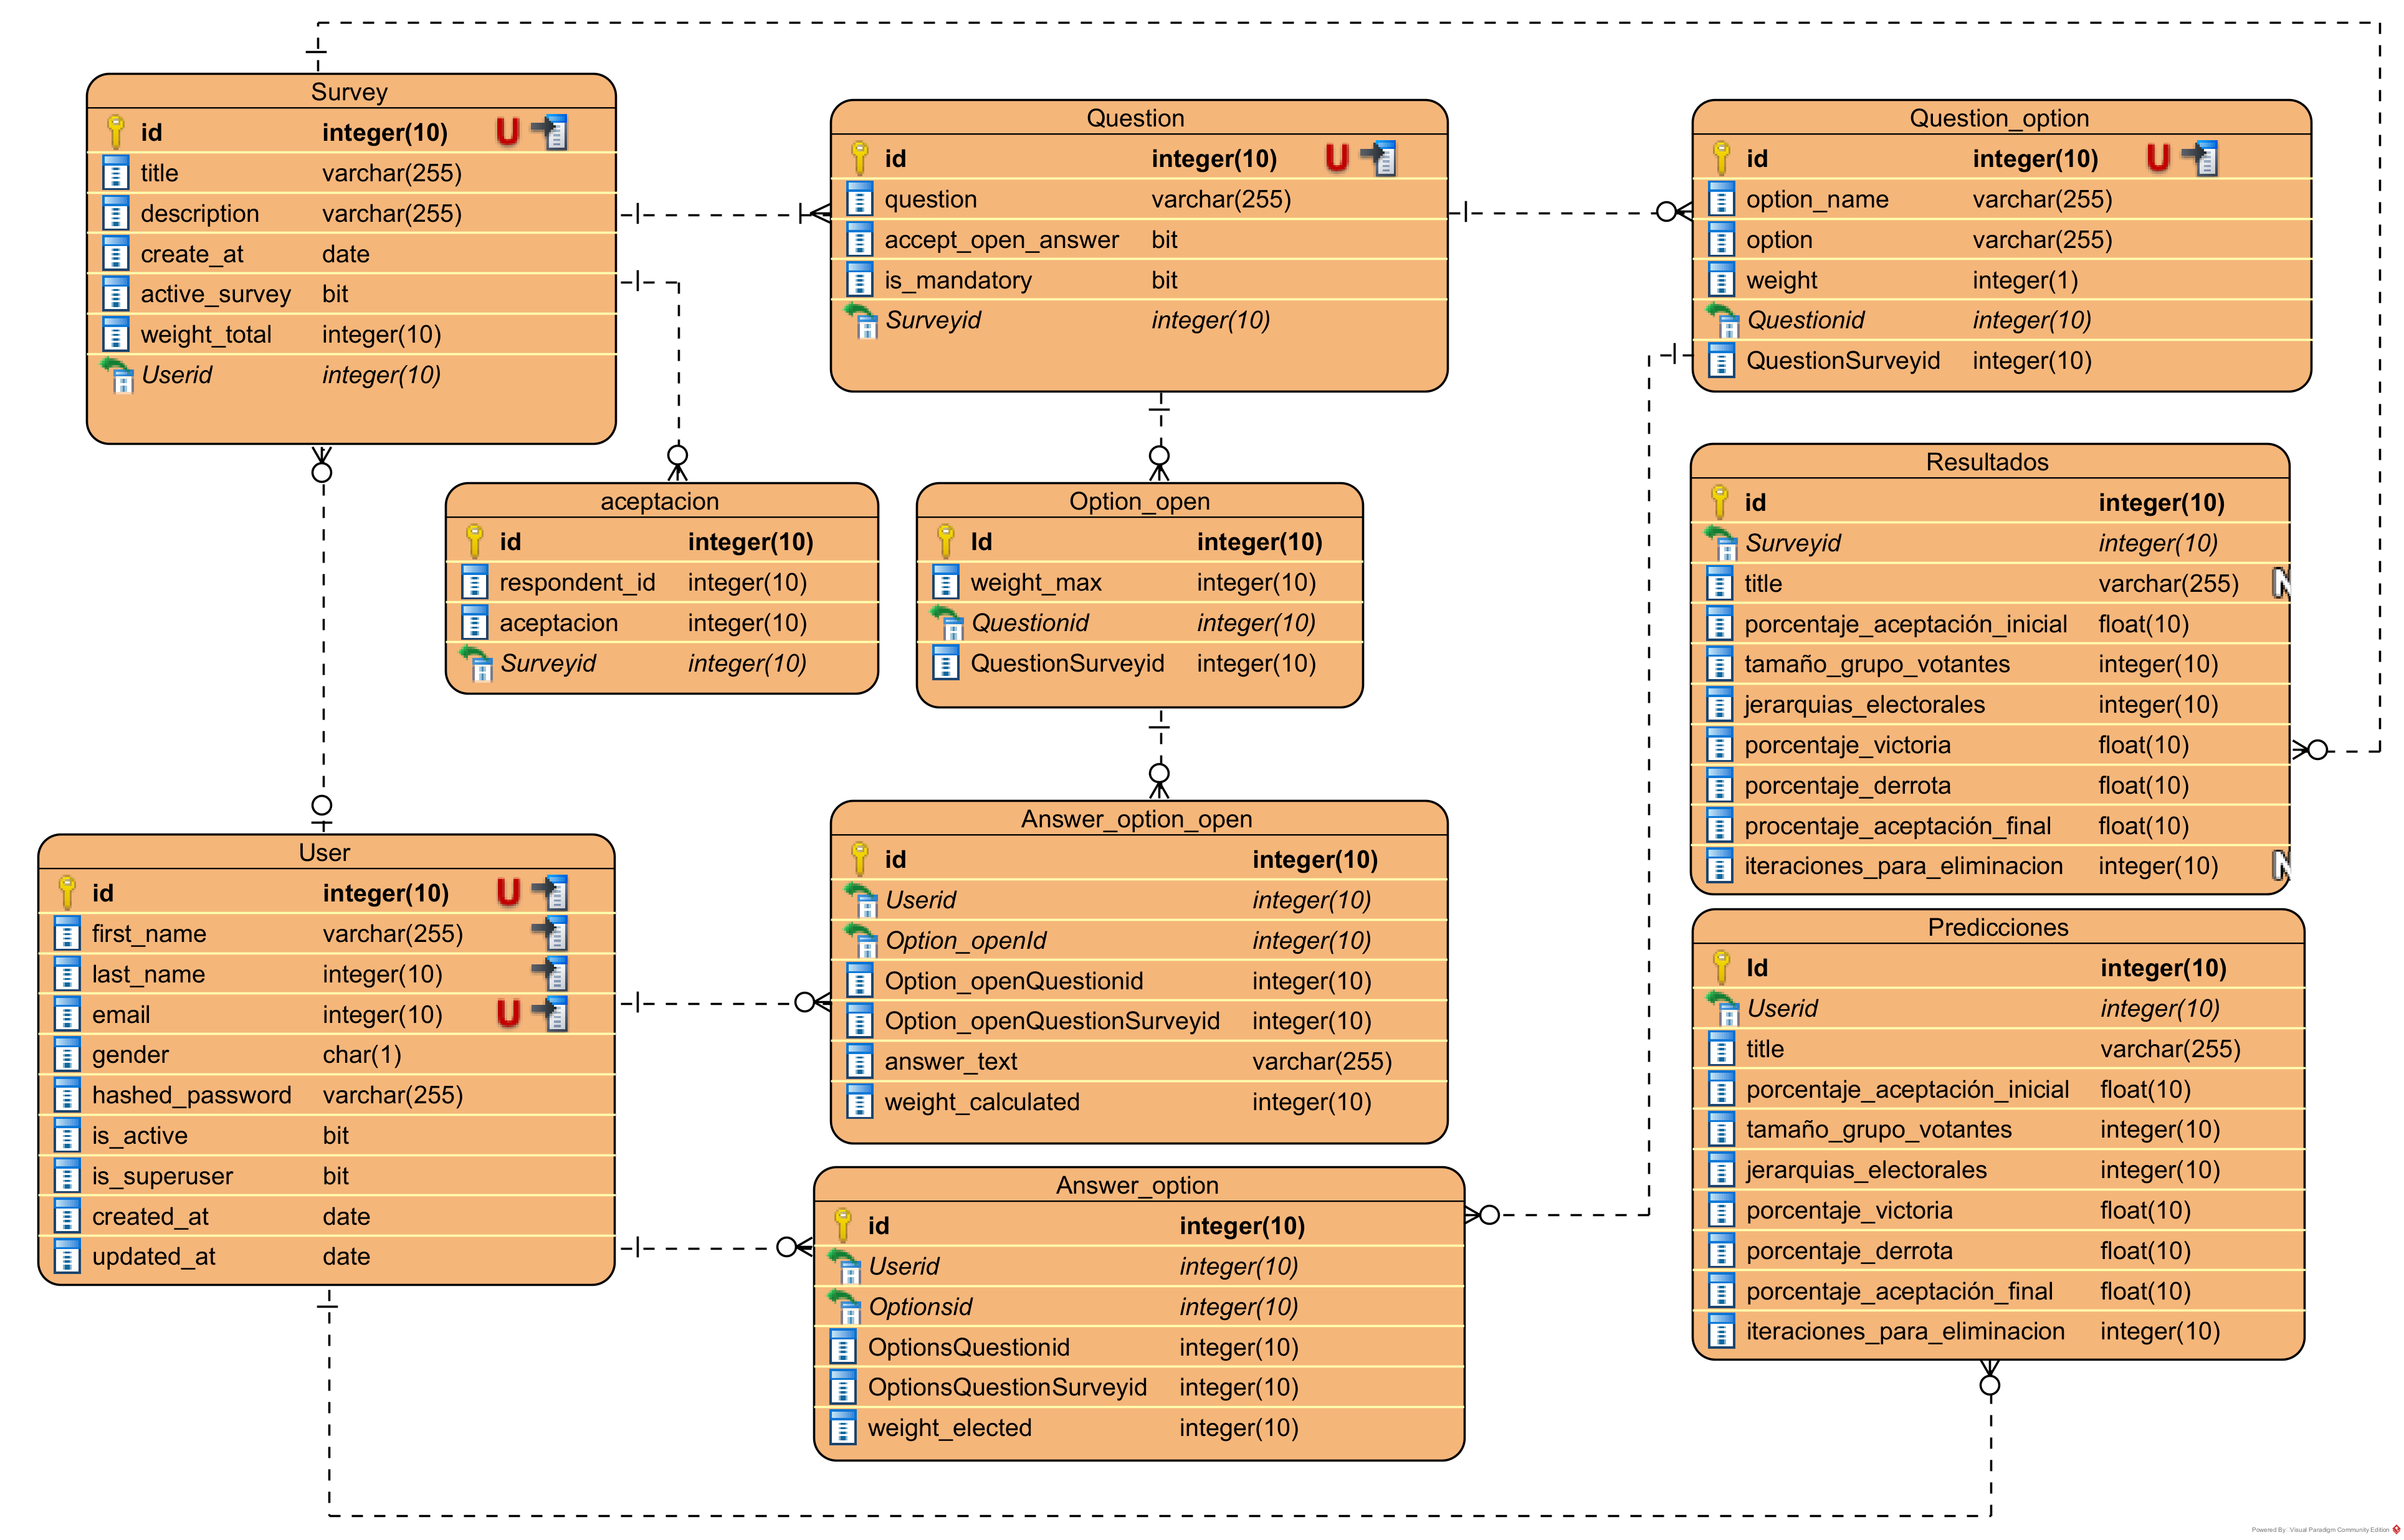
\includegraphics[scale=0.450]{TT/img/diseño/SISPREL.png}
    \caption{Diagrama entidad-relación de SISPREL}
    \label{graphic:entidad-relación}
\end{figure}

%\subsection{Modelo relacional}